\chapter{Le contrôle hormonal de la reproduction}\label{ch:b2:reproductive-hormones}

Chaque mois, selon un calendrier tenu à un ou deux jours près pendant
trente ans, un \omterm{def:b2:mammal-reproduction:ovary}{follicule} mûrit, un ovocyte est libéré, la muqueuse de
l'utérus s'épaissit puis, à moins qu'un embryon ne soit arrivé, se
désagrège. Aucune horloge du corps ne bat à ce rythme~; celui-ci émerge
d'un dialogue entre trois organes --- l'hypothalamus, l'hypophyse et
l'ovaire --- dans lequel chaque hormone commande la libération de la
suivante et la dernière commande la première. Ce chapitre démonte ce
dialogue~: l'axe qui gouverne les deux sexes, le contrôle tonique du
\omterm{def:b2:mammal-reproduction:testis}{testicule}, le contrôle cyclique de l'ovaire avec son remarquable
basculement d'une rétroaction négative à une rétroaction positive, et
les façons dont l'axe est court-circuité par la grossesse, par les
médicaments et par la médecine.

\section{L'axe}

\begin{definition}[L'axe hypothalamo-hypophyso-gonadique]\label{def:b2:reproductive-hormones:axis}
\index{gonadoliberine@gonadolibérine}\index{hormone luteinisante@hormone lutéinisante}\index{hormone folliculostimulante}\index{retroaction negative!hormonale@rétroaction négative!hormonale}
Des neurones de l'\emph{hypothalamus} sécrètent la \emph{GnRH}
(gonadolibérine, un peptide de dix acides aminés) dans les petits
vaisseaux portes qui descendent vers l'\emph{antéhypophyse}, sous forme
de brefs \emph{pulses} toutes les une à deux heures. La GnRH fait
sécréter par l'hypophyse, dans la circulation générale, deux hormones
glycoprotéiques, les \emph{gonadotrophines} \emph{LH} (hormone
lutéinisante) et \emph{FSH} (hormone folliculostimulante). Celles-ci
agissent sur les \emph{gonades}~: la LH sur les cellules productrices de
stéroïdes (\omterm{def:b2:mammal-reproduction:testis}{cellules de Leydig}, cellules de la thèque et du \omterm{def:b2:mammal-reproduction:ovary}{corps jaune}),
la FSH sur les cellules qui nourrissent les gamètes (\omterm{def:b2:mammal-reproduction:testis}{cellules de Sertoli}
et de la granulosa). Les gonades répondent par des stéroïdes ---
\emph{testostérone}, \emph{œstradiol}, \emph{progestérone} --- et par
un peptide, l'\emph{inhibine}, qui exercent une rétroaction sur
l'hypothalamus et l'hypophyse~: les stéroïdes sur les deux, surtout de
façon \emph{négative}~; l'inhibine sur la seule FSH. Il en résulte une
boucle régulée dans laquelle la production de la gonade est maintenue à
une valeur de consigne, et le même schéma à trois étages gouverne la
thyroïde et la corticosurrénale. Les mécanismes par lesquels ces
hormones agissent sur leurs cellules font l'objet du
\cref{ch:b2:cell-signalling}.
\end{definition}

\begin{omfigure}
\begin{tikzpicture}[every node/.style={font=\scriptsize}, >=stealth]
  \node[draw, rounded corners, fill=omDef!15, align=center, minimum width=3cm] (hyp) at (0,4.2) {hypothalamus\\GnRH, en pulses};
  \node[draw, rounded corners, fill=omDef!15, align=center, minimum width=3cm] (pit) at (0,2.2) {antéhypophyse\\LH et FSH};
  \node[draw, rounded corners, fill=omProp!20, align=center, minimum width=3cm] (gon) at (0,0) {gonade\\stéroïdes, inhibine};
  \node[draw, rounded corners, fill=omExo!25, align=center, minimum width=3cm] (tar) at (5.2,0) {tissus cibles\\gamétogenèse, voies génitales,\\caractères sexuels secondaires};
  \draw[->, thick] (hyp) -- (pit) node[midway, right] {vaisseaux portes};
  \draw[->, thick] (pit) -- (gon) node[midway, right] {sang};
  \draw[->, thick] (gon) -- (tar);
  \draw[->, thick, omThm] (gon.west) .. controls (-3.0,0) and (-3.0,2.2) .. (pit.west);
  \draw[->, thick, omThm] (gon.west) .. controls (-4.6,0) and (-4.6,4.2) .. (hyp.west);
  \node[omThm, anchor=east, align=right] at (-3.9,1.2) {vers l'hypophyse~:\\stéroïdes $(-)$,\\inhibine $(-)$ sur la FSH};
  \node[omThm, anchor=east, align=right] at (-3.9,3.6) {vers l'hypothalamus~:\\stéroïdes $(-)$\\(œstradiol $(+)$\\en milieu de cycle)};
\end{tikzpicture}

{\small L'axe~: la GnRH hypothalamique commande la LH et la FSH
hypophysaires, qui commandent la gonade~; les stéroïdes et l'inhibine de
la gonade exercent une rétroaction négative sur les deux étages
supérieurs --- sauf la brève rétroaction positive de l'œstradiol qui
déclenche l'\omterm{def:b2:mammal-reproduction:ovary}{ovulation}.}
\end{omfigure}

\begin{proposition}[Pourquoi les pulses comptent]\label{prop:b2:reproductive-hormones:pulses}
\index{secretion pulsatile@sécrétion pulsatile}\index{desensibilisation des recepteurs@désensibilisation des récepteurs}
L'hypophyse ne répond à la GnRH que si celle-ci arrive par pulses. Une
cellule exposée en continu à une hormone retire de sa surface les
récepteurs de cette hormone (\emph{désensibilisation})~; si le stock de
récepteurs est renouvelé à un taux $s$, éliminé à un taux basal $d$ et,
en présence de l'hormone $H$, à un taux supplémentaire $iH$, alors
\[
\frac{\mathrm{d}R}{\mathrm{d}t} = s - (d + iH)\,R, \qquad R^* = \frac{s}{d + iH},
\]
de sorte qu'un $H$ élevé et continu amène le nombre de récepteurs à un
état stationnaire bas et que la cellule se tait, tandis que de brefs
pulses séparés par des intervalles sans hormone laissent le stock se
reconstituer entre eux (constante de temps $1/d$). Un pulse de GnRH
toutes les quatre-vingt-dix minutes maintient l'hypophyse réactive~; une
perfusion continue, ou un agoniste de la GnRH à action prolongée, la met
au silence en quelques jours --- c'est le principe des médicaments qui
suppriment l'axe dans le cancer de la prostate, l'endométriose et la
puberté précoce. La fréquence des pulses code aussi une information~:
des pulses rapides favorisent la LH, des pulses lents la FSH.
\end{proposition}
\begin{proof}[Faits expérimentaux]
Knobil (1978--1980) détruisit les neurones à GnRH de singes rhésus, ce
qui abolit la LH, la FSH et le cycle, puis remplaça la GnRH à l'aide
d'une pompe~: un pulse par heure rétablit les gonadotrophines et des
cycles ovulatoires normaux~; la même dose journalière administrée en
continu les rétablit pendant quelques jours, puis la LH et la FSH
tombèrent à zéro~; le retour aux pulses les rétablit de nouveau. C'est
le mode d'administration, et non la quantité, qui constitue le signal.
\end{proof}

\begin{omfigure}
\begin{tikzpicture}
\begin{axis}[
  width=0.8\linewidth, height=5.4cm,
  axis x line=bottom, axis y line=left,
  xmin=0, xmax=40, ymin=0, ymax=1.2,
  xlabel={jours}, ylabel={LH plasmatique (relative)},
  xlabel style={font=\small, at={(axis description cs:0.5,-0.13)}, anchor=north},
  ylabel style={font=\small},
  tick label style={font=\small}, xtick={0,10,20,30,40}, ytick={0,0.5,1},
  clip=false,
]
\addplot[very thick, omDef, domain=0:10, samples=2] {1};
\addplot[very thick, omThm, domain=10:25, samples=60] {exp(-(x-10)/3)};
\addplot[very thick, omDef, domain=25:40, samples=60] {1-exp(-(x-25)/2)};
\fill[omDef!15] (axis cs:0,1.05) rectangle (axis cs:10,1.15); \node[font=\scriptsize] at (axis cs:5,1.1) {pulses horaires};
\fill[omThm!15] (axis cs:10,1.05) rectangle (axis cs:25,1.15); \node[font=\scriptsize] at (axis cs:17.5,1.1) {perfusion continue};
\fill[omDef!15] (axis cs:25,1.05) rectangle (axis cs:40,1.15); \node[font=\scriptsize] at (axis cs:32.5,1.1) {retour aux pulses};
\end{axis}
\end{tikzpicture}

{\small L'expérience de Knobil, schématisée. Chez un singe dont les
neurones à GnRH ont été détruits, des pulses horaires de GnRH
entretiennent la LH~; le passage à une perfusion continue de la même
quantité journalière l'éteint en quelques jours, et les pulses la
rétablissent.}
\end{omfigure}

\begin{omfigure}
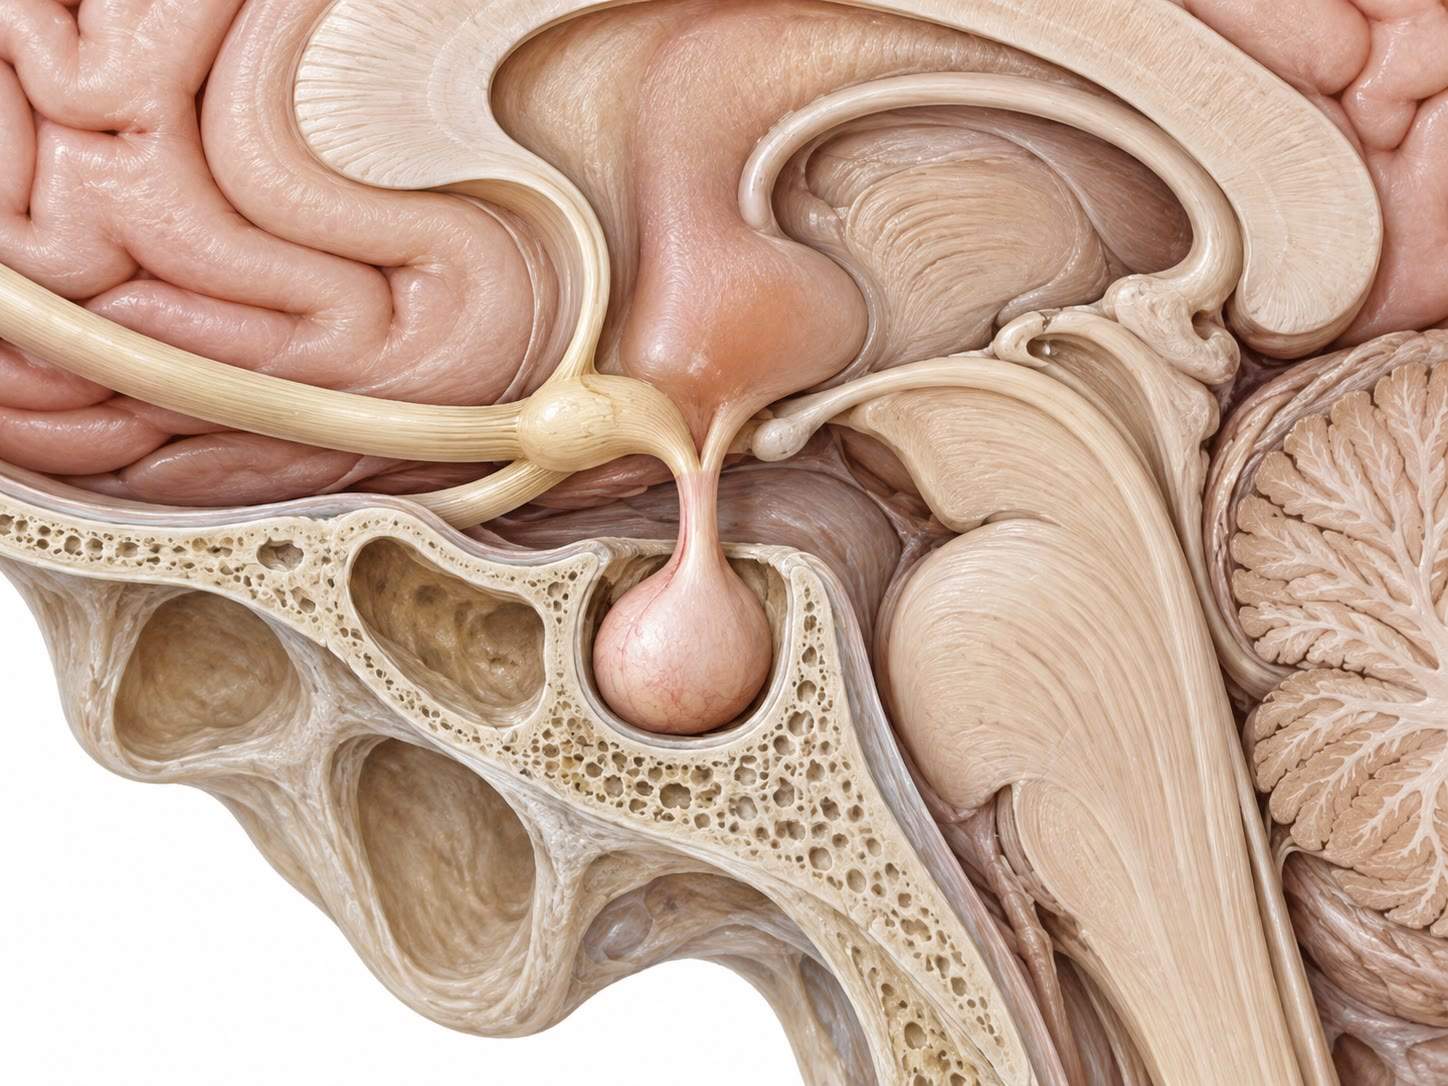
\includegraphics[width=0.55\linewidth]{images/book4/ai/b4-09-hypothalamus-pituitary.jpg}

{\small La base du cerveau en coupe sagittale~: l'hypothalamus au-dessus,
la tige pituitaire, et l'hypophyse dans sa loge osseuse --- le support
matériel de l'axe.}
\end{omfigure}

\section{Le mâle~: un contrôle tonique}

\begin{proposition}[Le contrôle du testicule]\label{prop:b2:reproductive-hormones:testis}
\index{testosterone@testostérone}\index{inhibine}
La LH agit sur les \omterm{def:b2:mammal-reproduction:testis}{cellules de Leydig}, qui produisent la
\emph{testostérone} (\qtyrange{3}{10}{ng/mL} dans le sang d'un homme
adulte, cent fois plus dans le \omterm{def:b2:mammal-reproduction:testis}{testicule}). La FSH agit sur les \omterm{def:b2:mammal-reproduction:testis}{cellules
de Sertoli}, qui --- avec la testostérone locale --- soutiennent la
\omterm{def:b2:mammal-reproduction:testis}{spermatogenèse} et sécrètent l'\emph{inhibine}. La testostérone exerce
une rétroaction sur l'hypothalamus et l'hypophyse qui freine la LH~;
l'inhibine exerce sur l'hypophyse une rétroaction qui freine la FSH.
Les deux boucles sont \emph{négatives} et le système est
\emph{tonique}~: les taux hormonaux fluctuent avec les pulses et au
cours de la journée (maximum le matin), mais ne sont pas cycliques, et
les spermatozoïdes sont produits en continu. La testostérone construit
et entretient aussi les glandes annexes et les voies génitales, la
barbe, la voix, les muscles et les os, la production d'hématies et la
libido, et chez le fœtus elle a construit le corps masculin
(\cref{ch:b2:mammal-reproduction}). La castration la supprime~: la LH et
la FSH sont multipliées par plusieurs faute de rétroaction, et les
caractères secondaires régressent~; la testostérone injectée restaure
les caractères --- mais pas la fertilité, car elle supprime aussi la LH
et donc la testostérone intratesticulaire qu'exige la \omterm{def:b2:mammal-reproduction:testis}{spermatogenèse}.
C'est pourquoi les stéroïdes anabolisants rendent les hommes stériles.
\end{proposition}
\begin{proof}[Faits expérimentaux]
Berthold (1849) castra des jeunes coqs~: leur crête rétrécit et ils
cessèrent de chanter et de se battre. Un \omterm{def:b2:mammal-reproduction:testis}{testicule} greffé dans
l'abdomen d'un castrat, où il se dota d'une nouvelle vascularisation
mais d'aucune innervation, restaura la crête, le chant et la
combativité~: le \omterm{def:b2:mammal-reproduction:testis}{testicule} agissait par le sang --- première
démonstration d'une sécrétion interne, cinquante ans avant le mot
hormone. La testostérone fut isolée et synthétisée en 1935.
\end{proof}

\section{La femelle~: un cycle avec un basculement}

\begin{definition}[Les cycles ovarien et utérin]\label{def:b2:reproductive-hormones:cycle}
\index{cycle menstruel}\index{phase folliculaire}\index{phase luteale@phase lutéale}\index{pic de LH}\index{endometre@endomètre}
Le cycle se compte à partir du premier jour des règles et dure environ
28 jours. \emph{Phase folliculaire} (jours 1--14)~: la FSH, libérée de
la rétroaction par la mort du \omterm{def:b2:mammal-reproduction:ovary}{corps jaune} précédent, recrute une
cohorte de \omterm{def:b2:mammal-reproduction:ovary}{follicules}~; ceux-ci sécrètent de l'\emph{œstradiol}, dont le
taux monte régulièrement~; l'œstradiol et l'inhibine abaissent la FSH,
et seul le \omterm{def:b2:mammal-reproduction:ovary}{follicule} qui possède le plus de récepteurs à la FSH survit
à cette baisse --- c'est le follicule dominant. Dans l'utérus,
l'œstradiol reconstruit l'\emph{endomètre} (phase proliférative) et rend
la glaire cervicale plus fluide. \emph{\omterm{def:b2:mammal-reproduction:ovary}{Ovulation}} (jour 14)~: lorsque
l'œstradiol s'est maintenu au-dessus d'environ \qty{200}{pg/mL}
pendant un jour et demi, sa rétroaction sur l'hypothalamus et
l'hypophyse bascule du négatif au \emph{positif}~; la LH est multipliée
par dix en une journée --- c'est le \emph{pic de LH} --- et environ
36 heures après son début, le \omterm{def:b2:mammal-reproduction:ovary}{follicule} se rompt et libère l'ovocyte.
\emph{Phase lutéale} (jours
15--28)~: le \omterm{def:b2:mammal-reproduction:ovary}{follicule} vidé devient le \omterm{def:b2:mammal-reproduction:ovary}{corps jaune} qui, sous l'effet de
la LH, sécrète de la \emph{progestérone} (\qtyrange{10}{20}{ng/mL}) et
de l'œstradiol~; la progestérone rend l'endomètre sécrétoire, épaissit
la glaire, élève la température basale de \qty{0.3}{\celsius} et, avec
l'œstradiol, freine la LH et la FSH. Le \omterm{def:b2:mammal-reproduction:ovary}{corps jaune} a une durée de vie
d'environ 14 jours~; à moins que l'hCG d'un embryon ne le sauve, il
régresse, la progestérone et l'œstradiol chutent, l'endomètre se
desquame (\emph{menstruation}), la FSH remonte et le cycle suivant
commence. La phase lutéale est fixe, de 14 jours~; la variation de la
durée du cycle est une variation de la phase folliculaire.
\end{definition}

\begin{omfigure}
\begin{tikzpicture}
\begin{axis}[
  width=0.94\linewidth, height=6.4cm,
  axis x line=bottom, axis y line=left,
  xmin=0, xmax=28, ymin=0, ymax=1.15,
  xlabel={jour du cycle}, ylabel={hormones (relatif au maximum)},
  xlabel style={font=\small, at={(axis description cs:0.5,-0.11)}, anchor=north},
  ylabel style={font=\small},
  tick label style={font=\small}, xtick={0,7,14,21,28}, ytick={0,0.5,1},
  legend style={font=\scriptsize, at={(0.5,-0.25)}, anchor=north, draw=none, legend columns=4},
  clip=false,
]
\addplot[very thick, omThm, domain=0:28, samples=120] {0.1 + 0.9*exp(-((x-14)^2)/0.9)};
\addlegendentry{LH}
\addplot[very thick, omProp, domain=0:28, samples=120] {0.35*exp(-x/6) + 0.15 + 0.35*exp(-((x-14)^2)/1.2)};
\addlegendentry{FSH}
\addplot[very thick, omDef, domain=0:28, samples=160] {0.1 + 0.9*exp(-((x-12.5)^2)/6) + 0.4*exp(-((x-21)^2)/12)};
\addlegendentry{œstradiol}
\addplot[very thick, omExo!70!black, domain=0:28, samples=160] {0.03 + 0.97*exp(-((x-21)^2)/12)*(x>14)};
\addlegendentry{progestérone}
\draw[dashed, gray] (axis cs:14.5,0) -- (axis cs:14.5,1.1); \node[font=\scriptsize, anchor=south] at (axis cs:14.5,1.1) {ovulation};
\node[font=\scriptsize, anchor=north] at (axis cs:7,1.1) {phase folliculaire};
\node[font=\scriptsize, anchor=north] at (axis cs:21.5,1.1) {phase lutéale};
\end{axis}
\end{tikzpicture}

{\small Les hormones du cycle. L'œstradiol produit par le \omterm{def:b2:mammal-reproduction:ovary}{follicule} en
croissance monte pendant la \omterm{def:b2:reproductive-hormones:cycle}{phase folliculaire} et, au-delà d'un seuil,
déclenche le \omterm{def:b2:reproductive-hormones:cycle}{pic de LH}~; l'\omterm{def:b2:mammal-reproduction:ovary}{ovulation} suit environ 36 heures plus tard~;
le \omterm{def:b2:mammal-reproduction:ovary}{corps jaune} sécrète ensuite de la progestérone pendant quinze jours,
puis meurt.}
\end{omfigure}

\begin{omfigure}
\begin{tikzpicture}[every node/.style={font=\scriptsize}]
  % endometrium thickness over the cycle
  \draw[thick, ->] (0,0) -- (12.4,0) node[right] {jour};
  \foreach \x/\l in {0/1, 2.1/5, 6.0/14, 12/28} \draw (\x,0.08) -- (\x,-0.08) node[below] {\l};
  \fill[omThm!25] (0,0) -- (0,1.4) .. controls (0.8,1.2) and (1.6,0.5) .. (2.1,0.35) -- (2.1,0) -- cycle;
  \fill[omDef!20] (2.1,0) -- (2.1,0.35) .. controls (3.5,0.6) and (5.2,1.3) .. (6.0,1.5) -- (6.0,0) -- cycle;
  \fill[omExo!35] (6.0,0) -- (6.0,1.5) .. controls (8,1.8) and (11,1.9) .. (12,1.6) -- (12,0) -- cycle;
  \node at (1.0,1.8) {règles};
  \node at (4.0,1.8) {proliférative (œstradiol)};
  \node at (9,2.2) {sécrétoire (progestérone)~: glandes, glycogène, artères spiralées};
  \node[anchor=east] at (-0.1,0.8) {endomètre};
\end{tikzpicture}

{\small Le cycle utérin. L'\omterm{def:b2:reproductive-hormones:cycle}{endomètre} se desquame lors des règles, se
reconstruit sous l'effet de l'œstradiol et devient sécrétoire sous
l'effet de la progestérone, prêt à recevoir un \omterm{def:b2:mammal-reproduction:implantation}{blastocyste} vers le
21\textsuperscript{e} jour~; quand la progestérone chute, il se
desquame de nouveau.}
\end{omfigure}

\begin{omfigure}
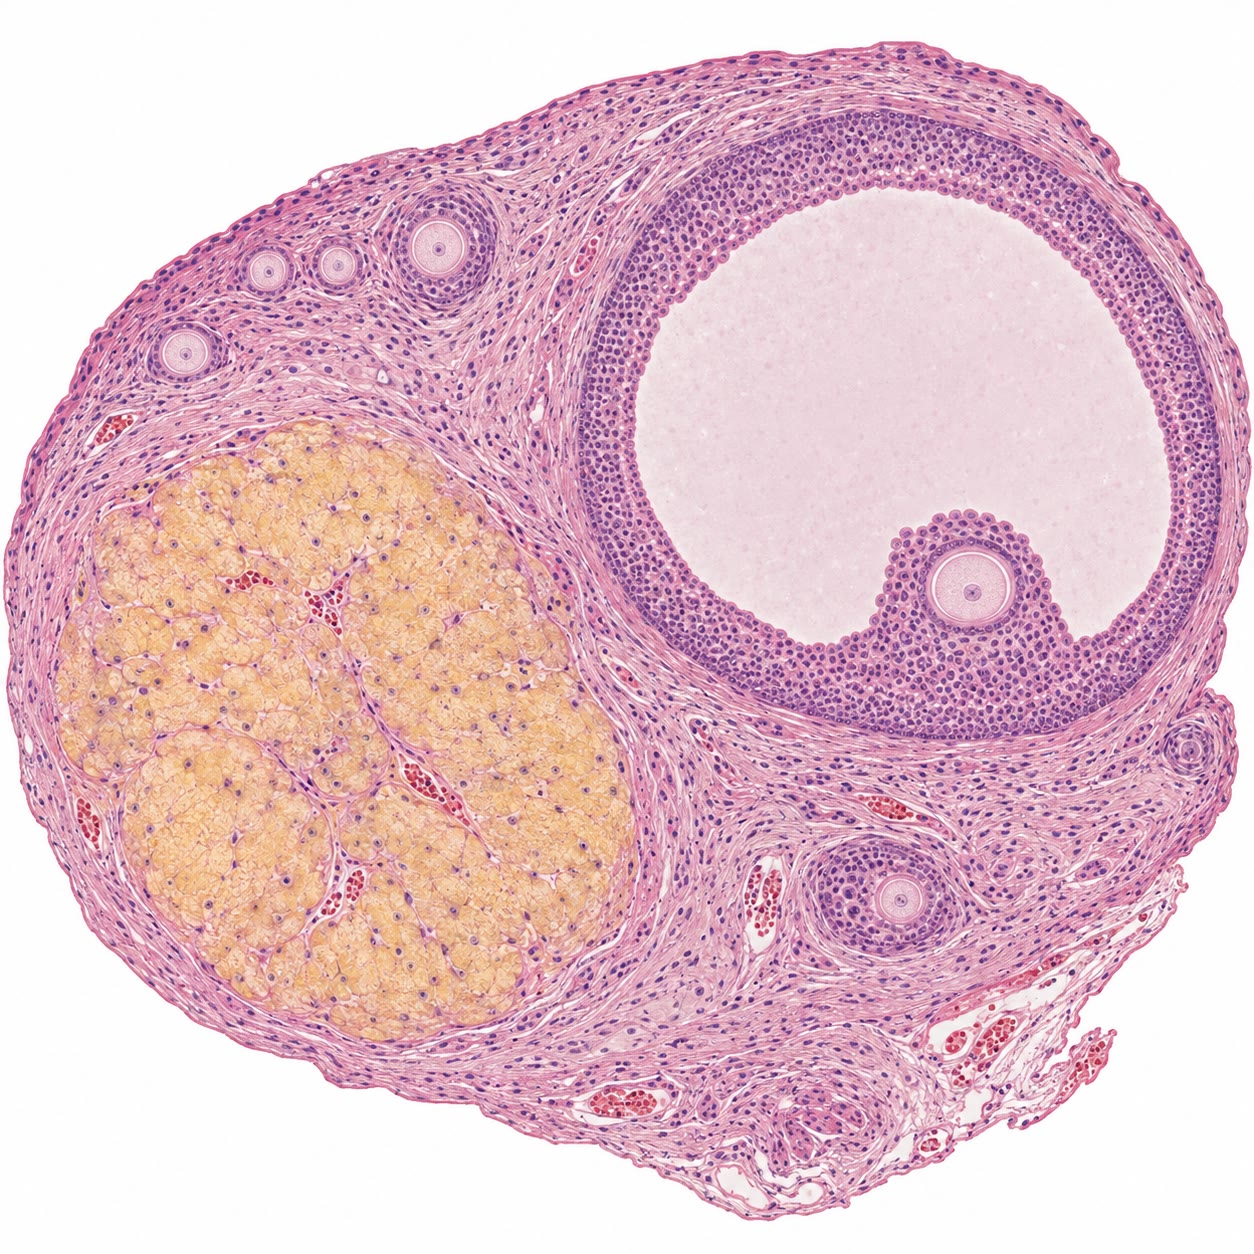
\includegraphics[width=0.46\linewidth]{images/book4/ai/b4-09-ovary-histology.jpg}

{\small Un ovaire en coupe~: un \omterm{def:b2:mammal-reproduction:ovary}{follicule} mûr avec sa cavité et son
ovocyte, de petits \omterm{def:b2:mammal-reproduction:ovary}{follicules} primordiaux sous la surface, et un \omterm{def:b2:mammal-reproduction:ovary}{corps
jaune} issu d'un cycle précédent.}
\end{omfigure}

\begin{theorem}[Le basculement de la rétroaction négative à la rétroaction positive]\label{thm:b2:reproductive-hormones:switch}
\index{retroaction positive!pic de LH@rétroaction positive!pic de LH}
L'œstradiol, aux faibles taux du début de la \omterm{def:b2:reproductive-hormones:cycle}{phase folliculaire}, inhibe
la LH et la FSH~; l'œstradiol au-dessus d'environ \qty{200}{pg/mL},
maintenu plus d'environ \qty{36}{h}, fait l'inverse~: il fait libérer
par l'hypothalamus une bouffée de GnRH et fait répondre l'hypophyse par
une multiplication par dix de la LH. Le mécanisme est un changement de
signe, et non de grandeur~: une dose élevée et prolongée induit dans
l'hypophyse un important stock de LH et une sensibilité accrue à la
GnRH, et dans l'hypothalamus (par l'intermédiaire des neurones à
kisspeptine) un basculement du générateur de pulses de GnRH en mode
pic. Ce basculement convertit un signal gradué --- la quantité
d'œstradiol que produit le \omterm{def:b2:mammal-reproduction:ovary}{follicule} --- en un événement tout-ou-rien
calé à la journée près, ce qu'exige l'\omterm{def:b2:mammal-reproduction:ovary}{ovulation}~; et comme seul un
\omterm{def:b2:mammal-reproduction:ovary}{follicule} grand et mûr peut maintenir \qty{200}{pg/mL}, le pic ne se
déclenche que lorsqu'un ovocyte est prêt à être libéré. Une fois
l'\omterm{def:b2:mammal-reproduction:ovary}{ovulation} survenue, la progestérone du \omterm{def:b2:mammal-reproduction:ovary}{corps jaune} rétablit la
rétroaction négative, et aucun second pic ne suit.
\end{theorem}
\begin{proof}[Faits expérimentaux]
Chez des femmes et des singes dont l'axe est freiné, une perfusion
d'œstradiol qui élève le taux plasmatique au-dessus de
\qty{200}{pg/mL} pendant deux jours est suivie d'un \omterm{def:b2:reproductive-hormones:cycle}{pic de LH}~; la même
quantité administrée pendant un jour, ou un taux plus faible pendant
trois jours, ne l'est pas. De la progestérone administrée avant la
perfusion bloque le pic~; administrée en même temps, elle l'avance et
l'amplifie. Ce seuil de dose et de durée reproduit le calendrier du pic
naturel à partir de la montée naturelle de l'œstradiol.
\end{proof}

\section{Court-circuiter le cycle}

\begin{proposition}[Grossesse, lactation, ménopause]\label{prop:b2:reproductive-hormones:overrides}
\index{hormone chorionique gonadotrope}\index{menopause@ménopause}
Un embryon en cours de \omterm{def:b2:mammal-reproduction:implantation}{nidation} sécrète l'\emph{hCG}, une hormone
analogue à la LH qui se fixe sur le récepteur de la LH et maintient le
\omterm{def:b2:mammal-reproduction:ovary}{corps jaune} en vie et en activité au-delà de ses quatorze jours~; vers
la dixième semaine, le \omterm{def:b2:mammal-reproduction:placenta}{placenta} produit lui-même assez de progestérone
et d'œstrogènes pour maintenir la grossesse, et le \omterm{def:b2:mammal-reproduction:ovary}{corps jaune} devient
superflu. Pendant toute la grossesse, les taux élevés de stéroïdes
maintiennent la LH et la FSH à zéro~: aucun \omterm{def:b2:mammal-reproduction:ovary}{follicule} ne croît, aucune
\omterm{def:b2:mammal-reproduction:ovary}{ovulation} n'a lieu. Après la naissance, la tétée élève la prolactine et
ralentit les pulses de GnRH, et l'\omterm{def:b2:mammal-reproduction:ovary}{ovulation} reste supprimée pendant des
mois. À la \emph{ménopause}, le stock de \omterm{def:b2:mammal-reproduction:ovary}{follicules} est épuisé~:
l'œstradiol et l'inhibine chutent et, faute de rétroaction, la LH et la
FSH montent à dix fois leur niveau antérieur et y restent --- la
signature d'une glande qui a cessé de répondre.
\end{proposition}

\begin{proposition}[Contraception et assistance médicale à la procréation]\label{prop:b2:reproductive-hormones:clinic}
\index{contraception!hormonale}\index{fecondation in vitro@fécondation in vitro}
La pilule combinée apporte chaque jour un œstrogène et un progestatif de
synthèse~: le taux constant de stéroïdes maintient la FSH et la LH
basses, aucun \omterm{def:b2:mammal-reproduction:ovary}{follicule} n'est recruté, aucune montée d'œstradiol ne se
produit, et le pic ne se déclenche jamais~; le progestatif épaissit
aussi la glaire cervicale. L'arrêt de sept jours laisse l'\omterm{def:b2:reproductive-hormones:cycle}{endomètre}
saigner~; l'oubli de pilules plus de deux jours de suite laisse la FSH
s'échapper, et un \omterm{def:b2:mammal-reproduction:ovary}{follicule} peut croître. La contraception d'urgence
retarde le pic de quelques jours par une forte dose de progestatif.
Dans la \emph{\omterm{prop:b2:reproductive-hormones:clinic}{fécondation in vitro}}, l'axe est commandé dans l'autre
sens~: de la FSH quotidienne pendant dix jours supplante la sélection
d'un follicule dominant unique et fait mûrir dix \omterm{def:b2:mammal-reproduction:ovary}{follicules} ou plus~; un
antagoniste de la GnRH empêche un pic spontané prématuré~; une injection
d'hCG remplace le pic, et les ovocytes sont recueillis 34 à 36 heures
plus tard, juste avant le moment où ils auraient été libérés~; ils sont
fécondés dans une boîte, et un ou deux embryons sont transférés, les
autres étant congelés. Chez l'homme, la testostérone exogène ou un
analogue de la GnRH supprime la \omterm{def:b2:mammal-reproduction:testis}{spermatogenèse} en supprimant la LH ---
c'est le principe d'un contraceptif hormonal masculin, toujours pas
commercialisé. Tout cela est l'axe de la première section, lu à
rebours.
\end{proposition}

\section{Exercices}

\begin{exercise}[$\star$]\label{exo:b2:reproductive-hormones:1}
Schématiser l'axe chez le mâle~: les trois étages, les quatre hormones,
les deux boucles de rétroaction, et les cellules sur lesquelles agit
chaque hormone.
\end{exercise}

\begin{exercise}[$\star$]\label{exo:b2:reproductive-hormones:2}
Donner les phases des cycles ovarien et utérin, avec leurs jours et
l'hormone qui domine chacune.
\end{exercise}

\begin{exercise}[$\star$]\label{exo:b2:reproductive-hormones:3}
Expliquer comment la pilule combinée empêche l'\omterm{def:b2:mammal-reproduction:ovary}{ovulation}, et pourquoi
des saignements surviennent pendant la semaine sans pilule.
\end{exercise}

\begin{exercise}[$\star$]\label{exo:b2:reproductive-hormones:4}
Qu'advient-il de la LH, de la FSH et des caractères sexuels secondaires
d'un mâle adulte castré~? Lesquels de ces effets la testostérone
injectée corrige-t-elle, et lesquels non~?
\end{exercise}

\begin{exercise}[$\star\star$]\label{exo:b2:reproductive-hormones:5}
Les pulses de GnRH surviennent toutes les \qty{90}{min} pendant la \omterm{def:b2:reproductive-hormones:cycle}{phase
folliculaire} et toutes les \qty{4}{h} pendant la \omterm{def:b2:reproductive-hormones:cycle}{phase lutéale}. Combien
de pulses par jour dans chaque cas~? L'hypophyse favorise la LH aux
pulses rapides et la FSH aux pulses lents~: quelle gonadotrophine
devrait augmenter la première à la mort du \omterm{def:b2:mammal-reproduction:ovary}{corps jaune}, et pourquoi
est-ce la bonne~?
\end{exercise}

\begin{exercise}[$\star\star$]\label{exo:b2:reproductive-hormones:6}
Convertir \qty{200}{pg/mL} d'œstradiol (masse molaire
\qty{272}{g/mol}) en \unit{pmol/L}, et \qty{15}{ng/mL} de progestérone
(\qty{314}{g/mol}) en \unit{nmol/L}. Combien de molécules d'œstradiol
un microlitre de plasma contient-il au seuil du pic~?
\end{exercise}

\begin{exercise}[$\star\star$]\label{exo:b2:reproductive-hormones:7}
Les cycles d'une femme durent 35 jours. Sachant que la \omterm{def:b2:reproductive-hormones:cycle}{phase lutéale} est
fixe, quel jour ovule-t-elle, et quels jours sont féconds si les
spermatozoïdes survivent trois jours et l'ovocyte un~? Pourquoi la méthode
du calendrier échoue-t-elle pour des cycles irréguliers~?
\end{exercise}

\begin{exercise}[$\star\star$]\label{exo:b2:reproductive-hormones:8}
Un embryon s'implante au 21\textsuperscript{e} jour d'un cycle de
28 jours, et son hCG, partant de \qty{1}{IU/L}, double tous les deux
jours. Le \omterm{def:b2:mammal-reproduction:ovary}{corps jaune} a besoin de quelques IU/L d'hCG au
26\textsuperscript{e} jour pour survivre. L'embryon est-il à temps~?
Que se passerait-il si la \omterm{def:b2:mammal-reproduction:implantation}{nidation} était retardée au
25\textsuperscript{e} jour~?
\end{exercise}

\begin{exercise}[$\star\star$]\label{exo:b2:reproductive-hormones:9}
Indiquer ce que l'expérience de Knobil a montré et ce qu'elle a exclu,
et prévoir l'effet sur la LH, l'œstradiol et l'\omterm{def:b2:reproductive-hormones:cycle}{endomètre} d'un agoniste
de la GnRH à action prolongée administré à une femme pendant un mois.
\end{exercise}

\begin{exercise}[$\star\star\star$]\label{exo:b2:reproductive-hormones:10}
Dans le modèle des récepteurs, prendre $s = 100$ récepteurs par heure,
$d =
\qty{0.5}{h^{-1}}$ et $iH = \qty{6}{h^{-1}}$ en présence d'hormone.
Calculer le nombre de récepteurs à l'état stationnaire sans hormone et
avec une hormone continue. Avec un pulse de deux minutes toutes les
heures, calculer le nombre de récepteurs perdus par pulse et la
fraction du déficit récupérée avant le pulse suivant, et en déduire le
niveau autour duquel le stock se stabilise.
\end{exercise}

\begin{exercise}[$\star\star\star$]\label{exo:b2:reproductive-hormones:11}
Une femme ménopausée a une LH et une FSH dix fois supérieures à celles
d'une jeune femme et un œstradiol très bas~; une femme porteuse d'une
tumeur hypophysaire sécrétant de la prolactine a une LH basse, un
œstradiol bas et pas de cycles~; une femme porteuse d'une tumeur de la
granulosa a un œstradiol élevé, une LH basse et pas de cycles.
Expliquer chaque profil à partir de l'axe.
\end{exercise}

\begin{exercise}[$\star\star\star$]\label{exo:b2:reproductive-hormones:12}
«~La même hormone inhibe puis déclenche le \omterm{def:b2:reproductive-hormones:cycle}{pic de LH}.~» Expliquer
comment l'œstradiol peut avoir ces deux effets, pourquoi l'\omterm{def:b2:mammal-reproduction:ovary}{ovulation}
exige un interrupteur plutôt qu'un variateur, et ce qui irait mal avec
un variateur.
\end{exercise}

\section{Problème~: un cycle mesuré}

\begin{problem}[{Problème du week-end --- des dosages hormonaux quotidiens
d'un cycle sont lus pour en tirer les phases, le jour de l'ovulation et
la fenêtre de fécondité~; le seuil du pic, l'horloge du corps jaune et le
sauvetage par l'hCG sont calculés~; le modèle des récepteurs explique
l'expérience de Knobil~; et l'axe est commandé à rebours en clinique,
jusqu'au jour de l'ovulation, à la durée de la phase lutéale, à la
fenêtre de fécondité et au seuil du pic}]
\label{pb:b2:reproductive-hormones:1}
Du sang a été prélevé certains jours du cycle d'une femme~:

\begin{center}
\small
\begin{tabular}{lcccccccccc}
\hline
jour & 1 & 5 & 8 & 11 & 12 & 13 & 14 & 15 & 21 & 27 \\
\hline
œstradiol (\unit{pg/mL}) & 40 & 60 & 110 & 210 & 260 & 310 & 220 & 150 & 160 & 50 \\
LH (\unit{IU/L}) & 5 & 5 & 6 & 7 & 8 & 20 & 65 & 15 & 4 & 4 \\
progestérone (\unit{ng/mL}) & 0.5 & 0.5 & 0.6 & 0.7 & 0.8 & 1.0 & 1.5 & 3 & 16 & 2 \\
température (\unit{\celsius}) & 36.4 & 36.4 & 36.4 & 36.4 & 36.4 & 36.4 & 36.4 & 36.5 & 36.8 & 36.7 \\
\hline
\end{tabular}
\end{center}

Les règles ont commencé au jour 1 et de nouveau au jour 29.

\medskip
\noindent\textbf{Partie I --- Lire le cycle.}
\begin{enumerate}
  \item Identifier les \omterm{def:b2:reproductive-hormones:cycle}{phases folliculaire} et lutéale à partir du
        tableau, avec l'hormone qui marque chacune.
  \item Quel jour le \omterm{def:b2:reproductive-hormones:cycle}{pic de LH} a-t-il culminé~? Quand l'\omterm{def:b2:mammal-reproduction:ovary}{ovulation}
        a-t-elle eu lieu~?
  \item Combien de temps a duré la \omterm{def:b2:reproductive-hormones:cycle}{phase lutéale}~? Est-ce cohérent avec
        la durée de vie du \omterm{def:b2:mammal-reproduction:ovary}{corps jaune}~?
  \item Expliquer le décalage de température et pourquoi il confirme
        l'\omterm{def:b2:mammal-reproduction:ovary}{ovulation} sans pouvoir la prédire.
  \item Quels jours l'œstradiol était-il au-dessus de
        \qty{200}{pg/mL}~? Relier cette durée au pic.
  \item Donner la fenêtre de fécondité de ce cycle (spermatozoïdes trois
        jours, ovocyte un jour).
\end{enumerate}

\medskip
\noindent\textbf{Partie II --- Des chiffres.}
\begin{enumerate}[resume]
  \item Convertir l'œstradiol du jour 13 en \unit{pmol/L}, et la
        progestérone du jour 21 en \unit{nmol/L}.
  \item De quel facteur la LH a-t-elle augmenté du jour 12 au jour 14~?
        Pourquoi retombe-t-elle si vite ensuite (la demi-vie de la LH est
        d'environ \qty{1}{h})~?
  \item Si le cycle suivant de cette femme avait une \omterm{def:b2:reproductive-hormones:cycle}{phase folliculaire}
        de 21 jours, quel jour ovulerait-elle et quelle serait la durée
        du cycle~?
  \item Un embryon s'implante 7 jours après l'\omterm{def:b2:mammal-reproduction:ovary}{ovulation}. Quel jour de ce
        cycle l'hCG apparaîtrait-elle et, en doublant tous les deux jours
        à partir de \qty{1}{IU/L}, quel taux atteindrait-elle au jour
        27~?
  \item Expliquer pourquoi la progestérone de \qty{2}{ng/mL} au jour 27
        montre qu'aucun embryon ne s'est implanté.
  \item Quelles auraient été les valeurs de progestérone et d'œstradiol
        au jour 27 s'il y en avait eu un~?
\end{enumerate}

\medskip
\noindent\textbf{Partie III --- Rétroactions et pulses.}
\begin{enumerate}[resume]
  \item Expliquer, à l'aide des signes des rétroactions, pourquoi la FSH
        est maximale au début du cycle et pourquoi un seul \omterm{def:b2:mammal-reproduction:ovary}{follicule}
        survit en général.
  \item Dans le modèle des récepteurs avec $s = 100$ par heure, $d =
        \qty{0.5}{h^{-1}}$, $iH = \qty{6}{h^{-1}}$, calculer $R^*$
        sans hormone et sous hormone continue.
  \item Un pulse dure \qty{2}{min}. Partant du $R^*$ non stimulé,
        combien de récepteurs un pulse élimine-t-il (utiliser
        l'approximation linéaire $iHR\,\Delta t$)~? Quelle fraction du
        déficit est récupérée pendant l'heure qui précède le pulse
        suivant (constante de temps $1/d$), et autour de quel niveau le
        stock se stabilise-t-il~?
  \item Utiliser ces chiffres pour expliquer le résultat de Knobil.
  \item Un homme reçoit en continu un agoniste de la GnRH pour un cancer
        de la prostate. Prévoir sa LH et sa testostérone au bout d'un
        jour et au bout d'un mois, et expliquer la différence.
  \item Les cellules de la granulosa d'une femme ne fabriquent pas
        d'inhibine. Prévoir sa FSH et sa LH, et la conséquence sur le
        recrutement folliculaire.
\end{enumerate}

\medskip
\noindent\textbf{Partie IV --- La clinique.}
\begin{enumerate}[resume]
  \item Pour une \omterm{prop:b2:reproductive-hormones:clinic}{fécondation in vitro}, cette femme reçoit de la FSH
        chaque jour à partir du jour 2. Expliquer pourquoi dix \omterm{def:b2:mammal-reproduction:ovary}{follicules}
        mûrissent au lieu d'un.
  \item Pourquoi ajoute-t-on un antagoniste de la GnRH à partir du
        jour 6, et que se passerait-il sans lui~?
  \item L'hCG est injectée quand les \omterm{def:b2:mammal-reproduction:ovary}{follicules} sont mûrs~; les ovocytes
        sont recueillis 35 heures plus tard. Justifier ce délai à partir
        du tableau.
  \item Dix ovocytes sont recueillis~; \qty{70}{\%} sont fécondés,
        \qty{40}{\%} des embryons atteignent le stade \omterm{def:b2:mammal-reproduction:implantation}{blastocyste}, et
        chaque \omterm{def:b2:mammal-reproduction:implantation}{blastocyste} transféré s'implante avec une probabilité de
        $0.35$. Nombre attendu de \omterm{def:b2:mammal-reproduction:implantation}{blastocystes}~? Probabilité d'au moins
        une grossesse si deux sont transférés~?
  \item Expliquer pourquoi la pilule combinée, prise par cette femme,
        aurait donné un tableau sans \omterm{def:b2:reproductive-hormones:cycle}{pic de LH} ni montée de la
        progestérone.
  \item Un contraceptif masculin fondé sur un antagoniste de la GnRH
        supprimerait aussi la testostérone. Que faut-il administrer en
        même temps, et pourquoi cela ne rétablit-il pas la production de
        spermatozoïdes~?
  \item Énoncer le résultat~: le jour de l'\omterm{def:b2:mammal-reproduction:ovary}{ovulation}, la durée de la
        \omterm{def:b2:reproductive-hormones:cycle}{phase lutéale}, la fenêtre de fécondité, et le seuil et la durée
        d'œstradiol qui ont déclenché le pic.
\end{enumerate}
\end{problem}
